\part{Détail des composants linguistiques retenus}

\chapter{Actionnalité, volition et locus de contrôle : une escapade sémantique}

Nous adoptons ici une approche en priorité « structurelle »  du langage, plutôt que sémantique, c'est-à-dire que nous nous limitons aux niveaux grammatical et syntaxique pour la majeure partie de notre analyse. L'idée est de se concentrer de préférence sur ce qui, dans la langue, manifeste l'état d'esprit qui la sous-tend, et qui guiderait supposément l'utilisation de ses composants les plus structurels indépendamment du contenu sémantique particulier exprimé par le locuteur.

Néanmoins, il semble qu'il faille mentionner quelques travaux antérieurs de nature sémantique, en ce qu'ils sont étroitement liés à notre question de recherche, et bien qu’ils présentent des limites qui justifieront, selon nous, une focalisation ultérieure sur les éléments les plus structurels du discours.

\section{Les limites d’une analyse par mot-clé}

Sur la base des travaux de Pietraszkiewicz\footnote{\cite{pietraszkiewicz_big_2019}}, une analyse lexico-sémantique exploratoire aurait pu consister à simplement compter, pour chaque groupe de répliques de personnages « haut »  et « bas » statut, la fréquence relative de tous les lemmes inclus dans son dictionnaire d’agentivité, comme a pu le faire Seligman dans son étude de la Bible\footnote{Seligman, M., Maymin, P., « Agency in the Bible » (2022)}.

\begin{table}[H]
\caption{Dictionnaire de l’Agentivité de Pietraszkiewicz}
\centering
\bigskip
\begin{tabular}{|p{0.8\linewidth}|}
    \hline
    Mots \\
    \hline
    able accomplish* accurac* accurate* achiev* acquir* actualiz* adaptab* adept* ambition* ambitious* aptitude* aptly aptness aspiration* aspire* aspiring assert* attain* authoritative* autonomous* autonomy capab* careful* choice choices clever* compet* completion confident confidently conquer* conscientious* contemplat* contend* contest* decid* decision* decisive* defeat* deliberat* dependable determin* difficult* do doable doing eager* earn earned earning earns easiness easy effective* efficien* effort* empowered enact* endeavor* establish established establishes establishing exact* expert* fail* fluen* freedom* freely goal goal-oriented goals importan* independ* individualist insight* intent* intuition intuitive* keen* know* liberties liberty logic* loner* made make makes making mastered masterful* mastering mastery motivat* need needed needing needs objectiv* obtain* opportun* overcame overcome overcomes overcoming persever* persist* persistent pioneer* practic* pragmat* prevail* pride prideful* priorit* proactive* productive* productivity proficien* prosper* proud* purpose* pursu* rational* realiz* rebel* recog* reliab* reputation* resilien* resolute* resolution resolv* responsib* reward* risk* savv* score scored scores scoring self self-* should* significant* skill skilled skillful* skills* smart smartly steadfast* strive* striving* struggl* stubborn* succeed* success* sure take takes taking tenac* think thinking thinks thought took tried tries triumph* trying unaided unyielding* vanquish* victor* will willing* willpower win winner* winning* wins wit wits witting* won won't you you'* your yours yourself \\
    \hline
\end{tabular}
 \label{Tab:dico_pietra}
\end{table}

\begin{table}[ht]
\centering
\bigskip
\renewcommand{\arraystretch}{1.5} % Adjust the value as needed
\begin{tabular}{|c|p{10cm}|}
    \hline
    Catégorie & Mots \\
    \hline
    Agentivité & tried, victory, knowing, wit, pride, obtain, willing, choice, thinking, purposes, freedom, resolved, needs, opportunity, easy, determined, doing, success, obtained, established, sure, taking, liberty, need, knowledge, making, purpose, able, self, took, known, think, thought, know, take, make, your, do, should, made \\
    \hline
    Efficacité & able, many, some, which, have, having, but, also, these, those \\
    Optimisme & things, good, joy, yet, hope (mais pas “no hope”) \\
    Imagination & desire, new, truth, true, false, ask, asked, know, known \\
    \hline
\end{tabular}
\caption{Les mots agentifs retenus par Seligman}
 \label{Tab:dico_seligman}
\end{table}
\newpage

\bigskip

Cette liste aurait d'ailleurs pu être complétée par les travaux de Rouhizadeh\footnote{\cite{rouhizadeh_identifying_2018}}, ce dernier ayant démontré qu'un locus de contrôle interne était associé à des verbes indiquant une « tentative » (\textit{attempt} en anglais), tandis qu'un locus de contrôle externe serait associé à des verbes de cognition, de manque, de sentiments et d'espoir : 

\begin{figure}[H]
\centering
    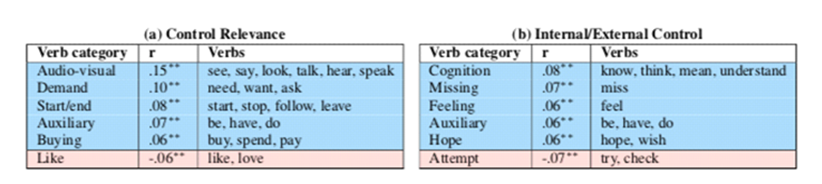
\includegraphics[width=16cm]{img/verbs_locus.png}
    \setlength{\abovecaptionskip}{-2pt} % Adjust the length to your preference
    \caption{Rouhizadeh et al. (2018) - Coefficients de régression logistique entre les catégories de verbes et le contrôle (les valeurs positives correspondent à la pertinence du contrôle et au contrôle externe). ** : p< 0,01 après correction de Benjamini-Hochberg. Les caractéristiques ayant des coefficients positifs sont en bleu et celles ayant des coefficients négatifs sont en rouge}
    \label{verbs_locus}
\end{figure}

Néanmoins, et outre le fait que ces études ont été menées en anglais et non en français, la principale limite d’une analyse sémantique réside dans sa vulnérabilité aux variations historiques de sens.

Certes, une analyse sémantique latente (LSA) aurait pu servir à calculer la similarité sémantique entre chaque mot unique d'un texte ou d'un énoncé, et un nombre limité de \textit{seed-words}\footnote{\cite{diuk_quantitative_2012}}, ce pour chaque groupe de répliques dans une pièce considérée. Il aurait également été possible de s’inspirer de la méthode « historiquement verrouillée »  de Snefjella\footnote{\cite{snefjella_historical_2019}}, afin de s'assurer de la stabilité sémantique, dans le temps, des \textit{seed-words} retenus.

Pour autant, ce travail dépassait largement le cadre de notre projet de recherche actuel, qu’il aurait fait reposer sur des méthodes d’analyse elles-mêmes exploratoires dans le cas de Snefjella. Aussi, notre paradigme et l’approche inspirée d’Hopper et Thompson\footnote{\cite{hopper_transitivity_1980}} justifiaient de se concentrer principalement sur les marqueurs linguistiques infra-sémantiques. 

\section{Les adverbes intentionnels, statut hybride ?}

La volition étant un aspect important de l'agentivité qu’il serait difficile d’analyser autrement que par une approche sémantique, nous avons cependant décidé de définir et de mesurer l'occurrence relative d'une liste d'adverbes univoquement intentionnels. Ceux-ci présentaient l'avantage d'être en nombre relativement limité dans la langue française, et d'avoir un sens \textit{a priori }historiquement stable.

\begin{table}[ht]
\caption{Expressions adverbiales à valeur intentionnelle retenues}
\centering
\bigskip
\renewcommand{\arraystretch}{1.5} % Adjust the value as needed
\begin{tabular}{|p{0.8\linewidth}|}
    \hline
     « volontairement », « délibérément », « expressément », « intentionnellement », « sciemment », « à dessein », « exprès »   \\
    \hline
\end{tabular}
 \label{Tab:adv_intention}
\end{table}

\section{La modalité : entre sémantique et pragmatique}

En guise de clôture de cette escapade sémantique, nous avons également examiné les marqueurs modaux utilisés dans les répliques de chaque groupe de personnages. 

La modalité est un concept linguistique qui s'intéresse au statut de la proposition décrivant l'événement\footnote{\cite{palmer_mood_1986}}, ou plutôt à l'attitude qu'un locuteur peut avoir vis-à-vis d'un événement ou d'un état. Une phrase modalisée situe une proposition sous-jacente, ou préjacente, dans l'espace des possibilités, décrivant des événements avec des informations supplémentaires telles que leur degré de désirabilité, de plausibilité ou de faisabilité.

Dans son sens le plus restrictif, la modalité est ainsi une « catégorie de signification linguistique ayant à voir [spécifiquement] avec l'expression de la possibilité et de la nécessité »\footnote{\cite{von_fintel_modality_2006}}.

On distingue traditionnellement deux grands types de modalité, qui nous intéressent particulièrement ici : la modalité épistémique (également appelée subjective ou hypothétique) et la modalité non épistémique, parfois appelée « orientée vers l'agent » (\textit{agent-oriented}), ou encore « racine déontique »  (\textit{deontic root}), « objective »  ou « pragmatique ».

La modalité épistémique concerne ce qui est possible, plausible ou nécessaire compte tenu de ce qui est connu et des preuves disponibles. Grâce à cette modalité, les locuteurs expriment un jugement sur le statut factuel de la proposition.

La modalité non épistémique est pour sa part composée de deux sous-modalités principales : l'une se concentrant sur les capacités objectives et le déroulement dynamique des événements (Palmer, 1986), parfois appelée  « modalité circonstancielle » ; et l'autre ayant avoir avec les raisons subjectives de donner la priorité à un événement plutôt qu'à un autre\footnote{\cite{portner_modality_2010}}, pour laquelle il existe d'autres subdivisions selon que l'événement est priorisé en termes de normes (« déontique »), de désirs/préférences (« boulétique »), ou de buts (« téléologique »).

A noter que Bybee et al.\footnote{\cite{bybee_evolution_1995}} ont élaboré leur propre classification s'agissant de la modalité « orientée vers l'agent », identifiant quatre sous-types : (i) l'obligation, (ii) la nécessité, (iii) la capacité et (iv) le désir. Ces auteurs discutent également d'un certain nombre de ressources pour représenter les connaissances des locuteurs ainsi que leur position à l'égard des événements et des états de fait. En particulier, l'utilisation de verbes modaux tels que les verbes anglais \textit{must}, \textit{should}, ou \textit{may} permettrait aux auditeurs de comprendre comment les locuteurs représentent leurs propres obligations ainsi que celles des autres dans un monde moral principalement construit par la langue (ou plutôt le discours). L'utilisation de prédicats de volition tels que \textit{want}, \textit{would}, \textit{would like}, ou \textit{wish}, pour leur part, mettrait certains états psychologiques internes à la disposition des autres pour qu'ils les comprennent et les évaluent. 

Ainsi, quelle que soit la taxonomie, la « modalité orientée vers l'agent » rend compte, par l'utilisation de verbes modaux en particulier, de l'existence de conditions internes et externes à l'accomplissement de l'action exprimée dans le prédicat principal. Avec cette définition, la modalité semble donc particulièrement liée à notre notion d’agentivité.

Cela étant, la modalité ultimement projetée par le locuteur, et/ou comprise par l'auditeur, dépend en réalité du contexte de l'occurrence, les verbes modaux seuls se révélant intrinsèquement polysémiques, ou du moins ambigus. A titre d’exemple, \textit{devoir} dans « Il devrait pleuvoir demain » a une connotation épistémique, tandis que « les visiteurs doivent partir à 6 heures »  est plutôt déontique, « Tu te dois d’y aller »  boulétique, « Pardon, je dois éternuer »  circonstancielle, et « Pour rentrer à temps, tu devrais prendre un taxi »  téléologique.

Pour déterminer la modalité d’une clause dans une perspective compositionnelle, Warsnby\footnote{\cite{warnsby_coding_2006}} détaille ainsi les caractéristiques, au-delà des verbes modaux et dans cet ordre de désambiguïsation, qui constitueraient ce qu'elle appelle la « contrôlabilité » du participant, définie comme « la capacité d'un agent à choisir de provoquer la situation référentielle représentée par les propositions des phrases »\footnote{\cite{klinge_impact_1996}}, et qui correspond étroitement à notre définition de l’agentivité, entendue dans un sens linguistique plus étroit. On précisera à nouveau que ces composantes ont été établies pour l'anglais seul. Cela dit, et compte tenu de l’inexistence de telles analyses appliquées au français, il semblait raisonnable d’y puiser une source d’inspiration, à supposer que leurs équivalents français soient interprétés de la même façon par des lecteurs francophones, ce à quoi ce mémoire tente précisément de répondre, \textit{in fine}.

Premièrement, la présence d'un adverbe de but (souvent une clause, comme dans « afin de [faire quelque chose] ») indiquerait une lecture non épistémique. Inversement, les adverbes modaux épistémiques tels que \textit{possiblement}, \textit{peut-être}, \textit{sûrement}, etc., peuvent qaunt à eux neutraliser, désambiguïser ou renforcer l'interprétation épistémique du modal dans un énoncé. Comme mentionné dans la section précédente, nous avons donc créé une mesure distincte pour les adverbes intentionnels, ainsi que pour les adverbes de doute et d'affirmation (chaque fois identifiés par l'usage d'expressions régulières).

\vspace{-40pt}

\begin{table}[H]
\caption{Expressions adverbiales à valeur de doute retenues}
\centering
\bigskip
\renewcommand{\arraystretch}{1.5} % Adjust the value as needed
\begin{tabular}{|p{0.8\linewidth}|}
    \hline
    « apparemment », « peut-être », « peut être », « probablement », 
    « vraisemblablement », 
    « éventuellement »,
    « supposément »,
    « présumément »,
    « possiblement »,
    « potentiellement »,
    « hypothétiquement »,
    « a priori », 
    « sans doute », 
    « si jamais »,
    « toutefois », 
    « certainement »   \\
    \hline
\end{tabular}
 \label{Tab:adv_doute}
\end{table}

\begin{table}[H]
\caption{Expressions adverbiales à valeur d'affirmation retenues}
\centering
\bigskip
\renewcommand{\arraystretch}{1.5} % Adjust the value as needed
\begin{tabular}{|p{0.8\linewidth}|}
    \hline
    « à vrai dire », « assurément », 
    « à coup sûr »,
    « absolument »,
    « bien sûr »,
    « pour sûr »,
    « sans conteste »,
    « sans contredit »,
    « bien entendu »,
    « effectivement », 
    « en effet »,
    « exactement »,
    « parfaitement »,
    « clairement »,
    « certainement »,
    « évidemment »,
    « fatalement »,
    « forcément »,
    « immanquablement »,
    « indubitablement »,
    « inéluctablement »,
    « inévitablement »,
    « infailliblement »,
    « sûrement »,
    « certes », 
    « en vérité », 
    « oui »,
    « précisément », 
    « sans doute », 
    « nul doute »,
    « sans aucun doute »,
    « sans le moindre doute »,
    « si fait », 
    « tout à fait »,
    « si. », « Si, », « Si : », « Si ! », 
    « soit. », « soit, », « soit : », « soit ! »,
    « volontiers », 
    « vraiment », 
    « naturellement », 
    « vraisemblablement »,
    « d'accord »   \\
    \hline
\end{tabular}
 \label{Tab:adv_affirmation}
\end{table}
\bigskip

En outre, la contrôlabilité sélectionnerait un agent non générique plutôt que générique, à savoir un agent animé, qui peut être approximé par les pronoms personnels (notamment au théâtre), ou un agent défini, approximé par le nombre de déterminants définis (bien que ce proxy soit très imparfait). Elle sélectionnerait également les événements (y compris les changements d'état), principalement interprétés comme déontiques, plutôt que les états (le plus souvent épistémiques), ce qui est encore une fois en alignement avec certaines de nos considérations théoriques au moment de sélectionner les marqueurs linguistiques de l’agentivité, notamment l’inclusion d’un ratio des verbes statifs par rapport aux autres verbes  (voir la partie \textit{III. 2.3. Analyse des dépendances syntaxiques}). A cela, nous ajoutons ainsi pour le calcul de l’indice agentif une métrique comptant le nombre relatif de pronoms personnels, ainsi qu’une métrique rapportant le nombre de déterminants définis à ceux indéfinis, sur la base des propositions de Warsnby.

Selon l’auteur, il s'agirait là des conditions explicites rendant inefficace l'influence d'autres caractéristiques.

Lorsqu’elles sont absentes, il est encore possible d’examiner les verbes modaux utilisés spécifiquement comme verbe matrice (c.a.d. principal) d'une clause de complément finie, qui reçoivent généralement une lecture épistémique. 

En outre, l'on peut supposer que les énoncés déontiques ont généralement une transitivité plus élevée que les énoncés épistémiques. Ceci est, une fois de plus, cohérent avec nos propres mesures (voir la partie \textit{III. 2.3. Analyse des dépendances syntaxiques}).

« Les situations situées dans le temps passé et les situations situées au moment de l'énonciation (progressives) seraient immuables, et donc hors du contrôle de l'agent », et interprétées comme épistémiques\footnote{\cite{klinge_impact_1996}}. Inversement, lorsque le temps de référence est postérieur au temps de la modalité exprimée, l'interprétation déontique serait possible (mais pas nécessaire). Il semblait toutefois trop complexe d’implémenter ce critère de façon efficiente, même en l’approximant.

En ce qui concerne la modification aspectuelle, la télicité sélectionnerait de préférence une interprétation déontique, et l'atélicité une interprétation épistémique. En particulier, le passé simple décrirait les événements en fonction du contexte (déontique), tandis que le passé composé ne donnerait qu'une information stative (épistémique). Comme cela est suggéré dans une autre partie de notre analyse (voir la section \textit{III. 2.2. Pronoms et déictiques : la référence au soi} notamment), nous avons inclus des métriques s'intéressant aux temps verbaux utilisés.

Enfin, la présence de la voix passive favoriserait une interprétation épistémique en indiquant un manque de contrôle de la part du sujet, mais aussi la stativité de la situation décrite, ce qui est encore une fois cohérent avec le lien entre  voix active et agentivité supposé plus bas (voir la partie \textit{III. 2.3. Analyse des dépendances syntaxiques}). 

 Warsnby note finalement que les énoncés contenant \textit{must}, (\textit{maste}), \textit{may} ou \textit{can} en anglais, dans lesquels les propositions sont codées de manière à indiquer un manque de contrôle de la part de l'agent, sont bien interprétés de manière épistémique. Dans les énoncés où les caractéristiques pertinentes indiquent que l'agent visé contrôle la situation dénotée par la proposition, en revanche, l'interprétation préférée est déontique.

Cela étant, nous n'avons en réalité pas pu analyser la modalité de manière compositionnelle comme nous le faisons pour la télicité (\textit{III. 3.1. L’analyse aspectuelle de la télicité}), en la définissant pour chaque clause spécifique, ce en raison d' un manque de temps et d'une trop grande complexification technique. Nous avons donc choisi d'estimer plutôt la modalité apparaissant comme la plus récurrente, au niveau global, dans chaque groupe de répliques, en se focalisant sur les verbes modaux, potentiellement modulés par les quelques proxys retenus plus haut. Ceci rend notre approche de la modalité particulièrement limitée, l’interprétation des verbes modaux étant dans une large mesure déterminée par l'ensemble de la construction dans laquelle ils s’inscrivent, à l’échelle de chaque clause. 

Il reste que l'on peut supposer de façon raisonnable que ces verbes modaux ont une signification préférentielle. En effet, une gradation intuitive semble exister entre les modaux signifiant une obligation (\textit{devoir}, \textit{avoir besoin de}, \textit{être supposé faire} etc. - tous ces éléments atténuant l'agentivité et se référant à un locus de contrôle externe), une possibilité (\textit{pouvoir}, notamment au conditionnel, \textit{être susceptible} de etc.), une capacité (\textit{être capable de}, \textit{pouvoir} à l'indicatif), un désir (\textit{vouloir} [que quelqu'un fasse quelque chose], \textit{désirer}, \textit{aimer}, \textit{souhaiter} au conditionnel notamment etc.) ou une action à venir (\textit{être sur le point de},\textit{ être en train de}, l'emploi du futur etc. - les marqueurs de futurité se chevauchent avec la modalité car ils impliquent une certaine forme d'incertitude). En outre, les modaux utilisés en référence à l'agent et aux règles ou normes (déontiques), qui nous intéressent particulièrement, semblent précisément revêtir les sens les moins ambigus\footnote{\cite{nesselhauf_mechanisms_2012}}.

Pour autant, et compte tenu de notre seconde question de recherche diachronique, il est nécessaire de s'assurer que ces corrélations sémantiques préférentielles sont à peu près stables dans le temps.

Dans plusieurs de ses études, Hilpert\footnote{\cite{hilpert_change_2016}; \cite{hilpert_disentangling_2021}} utilise la modélisation de l'espace vectoriel sémantique fondée sur les tokens pour déterminer si différents auxiliaires modaux peuvent être distingués en termes de profils dits « collocationnels » (ce que l'on appelle la « sémantique distributionnelle »), et si différents sens du même auxiliaire présentent des préférences collocationnelles divergentes.  

Il constate, pour l'anglais, que les paires quasi-synonymes d'expressions modales, telles que \textit{may} et \textit{might}, ou \textit{must} et \textit{have to}, diffèrent dans leurs caractéristiques distributionnelles. En outre, \textit{may} en particulier aurait subi un changement sémantique continu, s'éloignant des significations modales déontiques et des utilisations textuelles « impliquées » (\textit{involved} en anglais) pour se rapprocher des significations épistémiques et d'un degré plus élevé d'informativité. En bref, les collocats verbaux les plus fortement attirés par \textit{may} au XIX\ieme ~siècle se prêtent à l'expression d'un sens permissif, tandis que les collocats les plus fréquents dans les données plus récentes se combinent avec \textit{may} pour exprimer des possibilités. 

Plus généralement, les aires sémantiques qui contiennent des verbes aux significations abstraites et épistémiques seraient en augmentation. Cela étant, \textit{must}, par exemple, est encore utilisé relativement plus souvent avec un sens déontique. Aussi, Hilpert conclut qu'en tant qu'éléments hautement grammaticalisés, les auxiliaires modaux anglais présentent une assez grande variabilité collocationnelle, mais que sous la surface de cette variabilité, il existe une multitude d'associations qui lient conventionnellement une expression modale donnée à un ensemble particulier d'éléments lexicaux, ou un sens modal spécifique à un contexte linguistique particulier. Ainsi, bien qu'il existe des changements sémantiques, Hilpert peut affirmer que \textit{might}, \textit{must} et \textit{could} ont globalement plus de potentiel épistémique, tandis que \textit{can} et \textit{will} sont stables en termes de sens et déontiques. Pour sa part, \textit{would} demeure assez ambivalent. Alors que \textit{will} n'a pas d'équivalent direct en français, l'analyse du modal \textit{pouvoir} (équivalent de \textit{can}) semblait donc particulièrement pertinente pour notre question, en considérant qu’il possède, en français également, un sens déontique relativement stable.

Mais pour complexifier encore l'analyse, la corrélation de ces verbes modaux avec le degré d’agentivité personnelle, sur la base de la gradation mentionnée plus haut, n'est en réalité pas évidente. La tragédie grecque illustre bien cette inéquation. Bien qu'il s'agisse d'un cas limite du point de vue du locus de contrôle des personnages, apparemment manifestement externe puisque ces derniers sont soumis à la contingence divine (bien que l'on trouve déjà, dans certaines tragédies, des expressions ambiguës telles que le « désir de sacrifice » d'Agamemnon\footnote{\cite{vernant_j-p__vidal-naquet_p_mythe_2005}}), d’aucuns pourrait considérer que ces mêmes personnages identifient en réalité les vexations divines à leur propre destin (faisant tout le tragique de la pièce, précisément). De fait, ils construisent souvent des récits \textit{a posteriori} pour donner un sens à leurs souffrances, et expriment en ce sens une capacité à interpréter cette contingence dans des termes personnels, caractéristique d’un haut niveau d’agentivité.

De la même façon, comme le suppose Rymes\footnote{\cite{rymes_construction_1995}} dans une étude socio-linguistique s'attachant à analyser le discours de jeunes adolescents ayant abandonné l'école secondaire dans les années 90, pour continuer à se considérer comme de bonnes personnes malgré les actes criminels qu'ils ont commis, ces mêmes jeunes atténuent paradoxalement l'agentivité réelle induite par leur langage, principalement par l'utilisation de verbes modaux associés à un locus de contrôle externe, dans un acte qui pourrait pour sa part être considéré comme particulièrement agentif (ce que Rymes appelle « l'agentivité morale »).

C'est en ce sens que nous avons décliné notre métrique s’attachant aux verbes modaux de différentes manières. En trouvant les équivalents français les plus directs par recoupement de grammaires françaises bien connues et accessibles en ligne\footnote{\cite{jacqueline_ollivier_martin_beaudoin_grammaire_2007}; \cite{cedrick_fairon_maurice_grevisse_petit_2018}; \cite{delatour_nouvelle_1991}}, nous avons tout d'abord inclus une métrique comptant le nombre relatif de verbes modaux globalement utilisés, comme approximation de l’agentivité discursive ou morale des personnages considérés, ce quel que soit le contrôle sur l’action sémantiquement impliqué par le verbe modal en question. Nous avons en réalité calculé deux versions différentes de cet indicateur, l'une restrictive se concentrant sur les modaux d'obligation/permission et de désir (« pouvoir », « devoir », « vouloir », « falloir} + infinitif) et l'autre plus large (contenant également « espérer », « savoir », « penser », « aller » + infinitif). 

Nous avons également, au moyen d’une nouvelle métrique, opposé l'utilisation personnelle des modaux (à savoir ceux dont le sujet est à la première personne) à leur utilisation globale. En effet, cette utilisation « structurelle » des modaux, qui ne tient pas compte de leur contenu sémantique, pourrait n’être pertinente que lorsqu'on parle de soi (l’agentivité discursive ou morale se restreignant potentiellement aux seuls récits identitaires).

A cela, nous avons enfin ajouté une métrique calculant le rapport entre les modaux traduisant un locus de contrôle interne (« pouvoir », « vouloir » + infinitif), et externe respectivement (« devoir », « falloir » + infinitif), étant donné leur connotation agentive plutôt univoque et stable dans le temps, en tenant compte cette fois du contrôle sémantiquement impliqué par le modal employé. 

L’idée d’une utilisation des verbes modaux d'abord « performative », et en cela partiellement indépendante de leur contenu sémantique, est d'ailleurs corroborée par l'observation de tendances globales dans l'utilisation des verbes modaux, ayant affecté chacun d'entre eux de façon indistincte. De nombreux articles\footnote{\cite{myhill_change_1995}}\footnote{\cite{smith_changes_2003}}\footnote{\cite{leech_change_nodate}}\footnote{\cite{aarts_modals_2013}} ont en effet constaté un déclin général de la fréquence d'utilisation des verbes modaux au cours du XX\ieme ~siècle au moins, bien que ce phénomène pourrait être compensé par une augmentation globale parallèle de l'utilisation des verbes semi-modaux en anglais (à l'exception de \textit{have got to}). En particulier, ces travaux observent que \textit{will} et \textit{must} sont les verbes qui diminuent le plus drastiquement, tandis que l’utilisation de \textit{need} et \textit{be going to} (semi-modaux) augmente. Il s’agirait donc plutôt d'un glissement que d'une disparition pure et simple de la modalité. Pour autant, ce dernier souligne la limite de notre métrique comptant simplement le nombre total de verbes modaux utilisés, qui ne saurait se suffire à elle-même à l'heure où l'expression de la modalité se ferait plus discrète.

Plus problématique encore pour notre analyse, et comme le suggèrait Hilpert, il semblerait que l’on assiste au déclin du sens « intentionnel » (en anglais \textit{'speaker’s intention’-sense}) des modaux, notamment pour \textit{will}, ce en faveur d'un sens de « pure prédiction » (\textit{'pure-prediction’ sense}\footnote{\cite{nesselhauf_mechanisms_2012}}, sur la base de ses seules interprétations cependant, et d’un échantillon restreint d’expressions analysées), ce qui est cohérent avec le Bybee-path, aussi appelé processus de « grammaticalisation », une tendance inhérente à la langue dans son ensemble. Selon Bybee\footnote{\cite{bybee_evolution_1995}}, en cherchant à exprimer un sens plus spécifique, une langue finirait paradoxalement par « blanchir » (\textit{bleaching} en anglais), autorisant alors une plus grande acceptabilité contextuelle avec le temps, de sorte que de nombreuses significations se retrouvent à co-occuper dans un seul mot. Ainsi, plus une expression temporelle future est ancienne par exemple, plus elle exprimerait fréquemment une prédiction non colorée par la caractéristique de l'intention. Le déclin de l'expression de l'intention du sujet et du locuteur avec les marqueurs de futur résulterait donc de changements successifs entre les expressions de temps futur établies, et les nouvelles constructions venant prendre le relais pour exprimer les significations en question à mesure que les expressions de temps futur plus anciennes, du moins celles qui proviennent du matériel lexical, évoluent sur le chemin de Bybee pour exprimer la « prédiction pure ». 

Aussi, comme le note Nesselhauf\footnote{\cite{nesselhauf_mechanisms_2012}}, les deux types de changements sont probablement motivés, au moins en partie, par des transformations socioculturelles et stylistiques. En particulier, une explication souvent avancée pour rendre compte de ce moindre usage des verbes modaux, ou du moins de leur moindre explicitation des intérêts du locuteur, est celle de la « démocratisation de l'anglais » (les études ne s'intéressent là encore qu'à l’anglais seul). Cette dernière fait référence à une « montée d'alternatives plus conviviales et moins menaçantes, dans une société apparemment plus égalitaire, démocratique et antiautoritaire » qui conduirait à une « tendance des locuteurs à éviter les modes d'interaction inégaux », notamment les marqueurs manifestes d'autorité dans les énoncés véhiculant une directive (Farrelly et al., 2012). Cela expliquerait la préférence pour les modaux exprimant une obligation médiane, comme \textit{need to,} afin d'éviter les marqueurs de pouvoir excessifs tels que \textit{must}. Une construction de la forme \textit{X needs you to} serait ainsi interprétée comme un appel plutôt que comme un ordre direct, psychologisant par-là les directives (certains parlent de « pseudo-démocratisation »).

D’autres phénomènes pourraient encore soutenir, selon Nesselhauf, le déclin du sens intentionnel de \textit{will} en particulier. Tout d'abord, une expression qui n’est pas traditionnellement une expression de futurité mais avec un sens intentionnel similaire pourrait avoir remplacé l'utilisation d'expressions du futur avec ce sens dans certains contextes. En effet, il semble qu'en anglais, \textit{be going to} et le \textit{present progressive} aient remplacé \textit{will} et \textit{shall}, dans une certaine mesure, pour exprimer une prédiction fondée sur l'intention du sujet. En ce sens, nous avons inclus une métrique mesurant l'utilisation du progressif, correspondant en français à l’expression « être en train de [faire quelque chose] ». En outre, la construction \textit{want to} est identifiée par Nesselhauf comme un marqueur de futurité émergent, qui a commencé à être utilisé pour des prédictions fondées sur l'intention du sujet.

Autre possibilité avancée par l'auteur, ce déclin pourrait en partie s’expliquer par un changement stylistique global: alors que dans les exemples du XVIII\ieme ~siècle, le sujet des clauses intentionnelles (avec \textit{shall}) diffère du locuteur, de sorte que seule l'intention du locuteur et non celle du sujet est exprimée, en anglais actuel, il semble beaucoup plus probable que l'on choisisse une construction où le locuteur et le sujet sont totalement ou partiellement identiques (c'est-à-dire avec \textit{I} ou \textit{we}, en anglais, comme sujet – l’auteur compare par exemple \textit{My friendship to you shall be steady} avec \textit{I'm always going to be your friend}). Et cela refléterait une tendance plus générale à passer de modes d'expression impersonnels à des modes d'expression plus personnels dans de nombreux types de textes. La diminution globale de la construction passive va également dans ce sens\footnote{\cite{leech_change_nodate}} ; et il est intéressant de constater que c'est principalement au théâtre et dans la conversation fictionnelle que le déclin a eu lieu\footnote{toutes ces observations s'appuient sur le Corpus ARCHER : \url{https://www.projects.alc.manchester.ac.uk/archer/}}.

Enfin, comme l'indique Nesselhauf, « les personnages de fiction pourraient être de plus en plus représentés comme se sentant davantage déterminés par les circonstances extérieures et comme ayant le sentiment que leurs intentions personnelles et celles des autres ont moins d'influence sur ce que l'avenir pourrait leur apporter. Et cela pourrait refléter une évolution plus générale, qui ne se limite pas à la représentation littéraire : à mesure que le réseau d'interconnexions dans la société devient de plus en plus complexe et dense (cf., par exemple, Elias 2000), l'intention propre d'un sujet pourrait avoir moins d'influence sur les événements futurs ou du moins pourrait amener les sujets à supposer que c'est le cas ». Cette affirmation est particulièrement contradictoire avec nos propres hypothèses. Néanmoins, il faut d'abord noter que dans l'analyse de Nesselhauf, ce sentiment potentiel de moindre contrôle sur les événements futurs ne s'étend en réalité pas aux prédictions fondées sur des arrangements pour lesquels le sujet a été personnellement impliqué, ce qui semble difficilement explicable selon la lecture précédente.

A partir de là, et en maintenant la validité de notre analyse modale, nous proposons une interprétation alternative : plutôt qu’une moindre futurité dans l'intention moderne, qui dénoterait une perte réelle ou perçue de contrôle sur les événements futurs, on peut au contraire considérer que le futur est de plus en plus infusé par l'intention de l’agent, ce dernier étant de plus en plus capable de planifier. Le passage de modaux (y compris \textit{will}) précédemment dévolus à l'expression de la seule intention à des marqueurs de futurité, laissant à \textit{will} une connotation épistémique plus neutre, apparaît sous ce nouvel éclairage particulièrement évocateur. Suivant un principe d'économie lexicale, et l'intention étant supposément devenue une dimension psychologique de plus en plus pervasive, il semblerait naturel que la langue l'incorpore dans sa structure même, libérant ainsi de l'espace sémantique pour d'autres nuances moins directement évidentes pour les interlocuteurs, dans la logique du \textit{foregrounding} mentionné plus tôt.

Pour autant, cela limite à nouveau la portée de notre analyse modale. Si nous n'avons plus autant besoin de la modalité pour souligner la dimension intentionnelle d'une proposition, il se pourrait que l'utilisation de verbes modaux, aussi bien internes qu'externes, n'augmente pas avec le temps. Notre analyse modale vise donc dans un premier temps à déterminer s'il existe une différence significative entre les personnages de haut et de bas statut dans l'utilisation des verbes modaux, tandis que le sens de la corrélation, si corrélation il y a, demeure théoriquement incertain. C'est également pour cette raison que nous avons inclus dans nos métriques, et calculé séparément, l'emploi du temps futur.

Un autre marqueur modal plus secondaire, et pouvant traduire un manque d’assertivité, est l'ellipse, elle aussi ajoutée au calcul de notre indice.

\chapter{Les proto-marqueurs agentifs}

De tout ce qui précède, l’on comprend qu’il semblait pertinent de donner la prévalence aux marqueurs d’agentivité les plus « typiques » pour construire notre indice, et dont la corrélation avec la notion d'agentivité était \textit{a priori} indépendante de la composition des clauses dans lesquels ils s’insèrent.

\section{Le verbe, un indicateur ambigüe}

Le verbe peut être considéré comme le marqueur linguistique prototypique de l'agentivité\footnote{\cite{formanowicz_verbs_2017}}, dénotant une disposition objective à l'action ou, plus implicitement, un locus de contrôle interne. Une composante de notre indice agentif a donc consisté à mesurer la proportion relative de verbes dans chaque groupe de répliques. 

Néanmoins, et étant donnée notre acception relativement large de la notion d’agentivité, la direction de la corrélation pour ce proto-marqueur est en réalité incertaine. En effet, il s’agit également d’une partie du discours à connotation plus « concrète »\footnote{\cite{strik_lievers_linguistic_2021}}, à laquelle des agents « haut niveau » pourraient préférer l’utilisation de parties du discours plus abstraites (voir la partie \textit{III. 3.3. Les marqueurs corrélés d’abstraction}).

\section{Pronoms et déictiques : la référence au soi}

Comme mentionné au chapitre I., le choix d'un pronom à la première personne rapproche notre attention du soi\footnote{\cite{chung_psychological_nodate}}, par rapport à un pronom à la troisième personne (bien qu'il faille probablement faire une distinction entre les récits indirects à la troisième personne et ceux utilisant le style indirect libre, qui semble largement compenser la distance induite par le choix du pronom au niveau syntaxique et expressif). 

Néanmoins, la dimension orale du théâtre ne donnait pas accès au critère de choix d’une personne par l'auteur, pour faire parler son personnage. 

Cela étant, il restait possible de comparer l'utilisation relative des pronoms personnels individuels (première et deuxième personne du singulier) et collectifs (première et deuxième personne du pluriel) par les personnages-mêmes, en supposant qu'un ratio en faveur des premiers dénote une plus grande focalisation sur soi, et ainsi une agentivité plus « haut niveau ». 

Dans la même logique, le choix du temps principal du récit peut être interprété à l'aune du degré d'identification au personnage souhaité par le lecteur, et ultimement par l'auteur (dans la mesure où il répond à une demande du public, mais aussi parce qu'il peut lui-même chercher à vivre son personnage de manière plus intime), traduisant ainsi une plus ou moins grande focalisation sur soi. Là encore, la spécificité du genre théâtral obligeait à se limiter à l'analyse des temps utilisés par les personnages-mêmes, qui ont été comptés séparément (futur, présent, passé simple et imparfait - à savoir tous ceux dont nous disposions compte tenu des outils linguistiques utilisés).

Les déictiques constituent un autre point d'intérêt linguistique. Ceux-ci désignent des termes qui ne prennent leur sens qu'en fonction de la situation d'énonciation dans laquelle ils sont utilisés (c.a.d. le locuteur, le lieu et le moment d'énonciation), et dont la distance induite entre ce qui est mentionné et le « centre déictique » (le locuteur) peut être plus ou moins proche. Intuitivement, l'utilisation de déictiques proximaux (plus proches de soi) plutôt que distaux semble devoir être corrélée à une plus grande agentivité, toujours au sens d'une plus grande identification « à » l'action. Nous avons ainsi comparé l'utilisation relative, par chaque groupe de personnages, des marqueurs déictiques français proximaux « ceci », « voici », « -ci », « ici », « (-)deçà », « maintenant » ; par rapport aux marqueurs distaux « cela », « voilà », « (-)là », « (-)delà » et « alors ». 

\section{Analyse des dépendances syntaxiques : agentivité et voix grammaticales, verbes statifs, transitivité}

\subsection{Agentivité grammaticale}

D'un point de vue linguistique, la notion d'Agent, entendue comme rôle sémantique (voir I.2.1.\textit{ Transitivité et foregrounding : des indices corrélés de l'efficacité de l'action}) est essentiellement portée par le verbe et ne peut être réduite à la seule présence d'un sujet humain. Cependant, il semble qu’il y ait une corrélation constante entre le type de sujet utilisé et l’animation (\textit{animacy}) du participant, cette dernière étant une condition préalable à toute forme d'agentivité. Une façon d'approcher l'agentivité des locuteurs, en évitant toute analyse sémantique, consistait donc à examiner leur degré d’animation, lui-même véhiculé par le type de sujet utilisé. De fait, Ahearn\footnote{\cite{ahearn_language_2001}} constate l’existence d’un continuum récurrent d'« animation » allant des pronoms de première et deuxième personne (animation élevée) aux référents inanimés exprimés par des expressions nominales indéfinies (animation faible), comme synthétisé dans le graphique suivant : 

\begin{figure}[!ht]
    \centering
    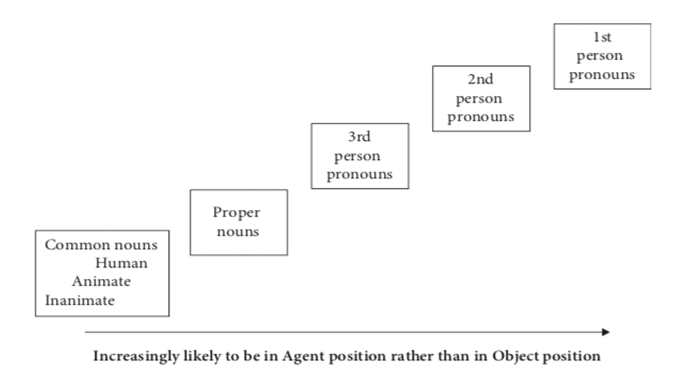
\includegraphics[width=16cm]{img/pronoun_animacy.png}
    \caption{Représentation des dénominations personnelles en fonction du degré d'\textit{animation} qu'elles évoquent - Ahearn (2001)}
    \label{pronoun_animacy}
\end{figure}

Là encore, la forme orale du théâtre rendait impossible l'utilisation de ce marqueur tel quel pour estimer l'agentivité du locuteur, puisque tous les personnages parlent à la première personne. Nous pouvions toutefois mesurer la proportion relative de pronoms à la première personne utilisés en position sujet, ou explicitement comme agents à la voix passive (en utilisant le \textit{parser} syntaxique de spaCy) dans chaque groupe de répliques, afin d’approximer très grossièrement leur agentivité grammaticale respective.

Pour la suite de l'analyse, et compte tenu de cette approximation très imparfaite, nous ne nous sommes pas limités à l'analyse des seules clauses dites « agentives » (celles comprenant un Agent au sens grammatical ou sémantique), mais nous avons plutôt dupliqué la mesure des indicateurs pour lesquels il était particulièrement difficile de savoir si leur relation avec l'agentivité dépendait du fait que le locuteur soit ou non le sujet de la clause, de la même façon que pour les verbes modaux. Nous avons ainsi dupliqué les mesures suivantes : verbes, copules, ratio de l'utilisation de la voix active vs. passive.

A titre de remarque, la gradation mentionnée ci-dessus a encore été utilisée dans l'analyse de la télicité : un personnage plus agentif pourrait en effet également être amené à prêter plus d'agentivité aux autres personnages qu'il ou elle mentionne, et ainsi à utiliser relativement plus de pronoms dénotant une animation particulière y compris lorsqu'il ou elle se réfère à d'autres individus. Il semble de fait qu'il existe un biais cognitif généralisé favorisant l'interprétation télique d'une phrase lorsqu'elle contient un sujet animé, et inversement une interprétation atélique dans le cas d'un sujet inanimé\footnote{\cite{graf_interaction_2017} - il s'agit là d'une études psycholinguistique, et non simplement théorique}. De manière cohérente, de nombreuses recherches indiquent que les entités inanimées sont incompatibles (ou du moins relativement moins compatibles que les entités animées) avec les verbes qui connotent l'intentionnalité, la planification ou impliquent des processus cognitifs, car ces entités inanimées n'ont pas les moyens de mener à bien des actions intentionnelles (voir ci-après).

\subsection{Voix active vs. passive}

Dans le même ordre d'idée, bien que cette fois-ci non soutenue par des travaux antérieurs, l'utilisation d'une voix active plutôt que passive (et malgré l'agentivité grammaticale qu'implique cette dernière) nous a semblé devoir être corrélée avec un degré d'agentivité plus élevé\footnote{\cite{hopper_transitivity_1980}}.

\subsection{Verbes statifs}

Un type de verbe pourrait constituer une exception univoque au lien verbe-agentivité : les verbes statifs ou d'état, qui se réfèrent principalement aux états émotionnels (et potentiellement durables) des agents, plutôt qu'à des actions. Il est vrai que l'on peut considérer les verbes exprimant des attitudes et des sentiments propositionnels comme évoquant des formes d'action mentale. Cependant, les \textit{verba sentiendi} (verbes de perception) sont généralement considérés comme moins « actifs ». 
Une autre composante linguistique de notre indice agentif a donc consisté à comparer la proportion relative de verbes purement statifs (ici approximés par l’utilisation des verbes \textit{être} et \textit{avoir} en excluant les emplois temporels, ainsi que par l'étiquette « copule » du \textit{parser} spaCy, les deux métriques étant mesurées séparément) par rapport aux verbes dits « dynamiques » (tous les autres verbes).

En guise de commentaire, et malgré leur supposée « stativité », l'utilisation du progressif avec des verbes d'émotions comme \textit{aimer} (par opposition à \textit{savoir}) semble en réalité être de plus en plus autorisée dans le langage courant, au moins à partir du XIX\ieme ~siècle pour l’anglais\footnote{\cite{granath_im_2014}}. Par ailleurs, Granath et al. notent qu'une telle combinaison entraînerait un changement aspectuel, suggérant alors une « agentivité accrue ». Cela remet en cause l'idée même d'une séparation binaire entre verbes statifs et non statifs, ces derniers se plaçant plutôt sur un continuum. De la même façon en effet, certains verbes appartenant traditionnellement à la catégorie des verbes dynamiques, notamment en référence à des activités et des événements physiques, se produisent rarement avec l'aspect progressif (par exemple \textit{shrug}, \textit{smash}, \textit{suck} et \textit{throw} en anglais). Notre analyse binaire est donc limitée, mais une approche tripartite, voire par degré de stativité, nécessitait de recourir à de la modélisation\footnote{\cite{klavans_degrees_1992}}\footnote{\cite{friedrich_automatic_2014}}\footnote{\cite{sims_literary_2019}}, ce qui dépassait le cadre technique de cette analyse. Aussi, nous avons tout de même mesuré l'usage relatif du progressif, considéré comme une indication potentiellement plus fine que l'opposition verbes statifs/autres verbes du dynamisme connoté par les événements, et indirectement de l'agentivité du locuteur (comparez simplement « je mange » avec « je suis en train de manger »).

\subsection{Transitivité}

Comme mentionné plus haut (I.2.1. \textit{Transitivité et foregrounding : des indices corrélés de l'efficacité de l'action}), la transitivité semble assez intuitivement liée à une perspective plus agentive, dans la mesure où le locuteur conçoit la possibilité d'une action directe sur un objet (grammatical). Une mesure de la proportion relative des verbes utilisés transitivement, plus proches de notre prototype de causalité\footnote{\cite{konopasky_towards_2016}}, a donc logiquement été ajoutée à notre indice.

\chapter{Traverser les distances psychologiques : l’agentivité et la planification}

Les gens sont capables de penser à l'avenir, au passé, à des endroits éloignés, à la perspective d'une autre personne et à des alternatives contrefactuelles. Sans nier le caractère unique de chaque processus, Trope et al.\footnote{\cite{trope_construal-level_2010}} ont proposé qu'ils constituent des formes différentes de franchissement d'une certaine distance psychologique. Selon eux, la distance psychologique est égocentrique : son point de référence est le soi, ici et maintenant (voir sur ce point la partie \textit{III. 2.2. Pronoms et déictiques : la référence au soi}), et les différentes façons dont un objet peut être éloigné de ce point (dans le temps, dans l'espace, dans la distance sociale et dans l'hypothéticité) constituent différentes dimensions de la distance. 

Aussi, plus les événements sont éloignés de l'expérience directe, plus ils sont susceptibles d'être représentés en des termes abstraits traduisant l'essence perçue des événements (constructions de haut niveau), plutôt qu'à travers les détails plus concrets et accessoires des événements (constructions de bas niveau), ce qui correspond étroitement à notre définition du continuum agentif. Cela est d'ailleurs corroboré par l’association, trouvée chez Woike\footnote{\cite{woike_use_1994}}, entre agentivité et différenciation (qui s'oppose au processus cognitif d’intégration\footnote{Les termes « séparé » et « connecté » ont souvent été utilisés pour décrire
deux conceptions différentes de l'individu par rapport au monde social : l'une comme autonome, indépendante et séparée des autres, et l'autre comme relationnelle, interdépendante et indépendante des autres. Pour Woike, cela suggère qu'il existe des processus cognitifs spécifiques impliqués dans la promotion et le maintien de ces deux orientations : la différenciation, qui consiste à percevoir un certain nombre d'aspects différents dans un groupe de stimuli donné, et l'intégration, qui consiste à établir des connexions ou des liens entre des stimuli différenciés}) : 

\begin{displayquote}
 « Parce que la différenciation implique de percevoir des différences et l'indépendance entre les attributs des stimuli sociaux, elle peut être utilisée plus fréquemment par les personnes qui ont une orientation vers l'individualisme et l'indépendance, car elle remplit une fonction particulière pour elles. Par exemple, Belenky et al. (1986) ont suggéré que la distance psychologique peut être maintenue en séparant le soi des objets sociaux afin de percevoir les choses de manière objective ou comme n'ayant aucun rapport avec soi. En outre, la pensée critique et la prise de décision sont, par définition, des procédures de comparaison qui impliquent de voir les différences relatives entre les choses. L'acte de séparer une question en la décomposant en plusieurs parties et en percevant ses contrastes et ses distinctions peut aider les percepteurs à porter des jugements et à prendre des décisions en limitant leur implication personnelle dans le contexte interpersonnel, ce qui leur permet de conserver une orientation individualiste. »
\end{displayquote}

Le degré de planification ou de capacité rétrospective de l'agent évoqués par une clause est ainsi une autre caractéristique linguistique importante.

\section{L’analyse aspectuelle de la télicité}

La télicité, ou « délimitation aspectuelle », est la propriété aspectuelle d'une phrase verbale (ou de la phrase dans son ensemble) qui indique qu'une action ou un événement a une fin spécifique. Du grec \textit{telos}, elle désigne plus précisément la « présence d'une finalité, intrinsèque ou envisagée, inhérente à l'événement, qui se manifeste mutuellement dès le moment où la situation a commencé et est évoquée », et au-delà de laquelle l'événement ne peut plus se poursuivre\footnote{\cite{depraetere_telicity_2007}}. A titre d’exemple, « courir vers quelqu'un » est considéré comme ayant un aspect plus télique que « jouer dans l'herbe » ou encore « marcher près d'un lac ».

Par définition, la télicité est donc liée à l'intentionnalité de l'agent. La manière dont un événement est évoqué (et réciproquement interprété) comme étant doté d'une valeur aspectuelle plus ou moins télique peut donc nous informer en partie quant à la mesure dans laquelle le locuteur se représente lui-même, ou ses \textit{alter ego}, comme capable d'agir volontairement sur le monde, par opposition à une idéologie plus fataliste par exemple. La télicité a donc également avoir, et ce d'une manière encore plus structurelle et compositionnelle, avec la notion d’agentivité. 

En nous inspirant de modèles d'apprentissage automatique de la télicité d'une clause (cités ci-après), qui donnaient accès aux principales caractéristiques utilisées par l'algorithme de classification (et dont la pertinence pour un lecteur humain était systématiquement vérifiée par la théorie linguistique ou par des études psycholinguistiques ultérieures), nous avons défini un certain nombre d'éléments linguistiques qui semblaient être décisifs dans la détermination de la télicité d'une phrase. Cette fois, et contrairement à la modalité, l'analyse se fait au niveau de la phrase-même (voire de la clause), puisque la télicité est définie de manière intrinsèquement compositionnelle (de telle sorte qu'une approximation au niveau des répliques concaténées des personnages n’avait pour le coup pas grand sens). En effet, si elle va souvent de pair avec les prédicats de réalisation et d'accomplissement, pour reprendre la classification de Vendler\footnote{\cite{vendler_verbs_nodate}: Les activités et les accomplissements se distinguent des réalisations et des états dans la mesure où les deux premières permettent l'utilisation d'aspects continus et progressifs. Les activités et les accomplissements se distinguent les unes des autres par leur délimitation. Les activités n'ont pas de point final (un point avant lequel l'activité a eu lieu et après lequel elle ne peut plus continuer, comme pour « Jean a dessiné un cercle »), alors que les accomplissements en ont un. En ce qui concerne les réalisations et les états, les réalisations sont instantanées, mais les états sont durables. Les réalisations et les accomplissements se distinguent l'un de l'autre par le fait que les réalisations ont lieu immédiatement (comme dans « reconnaître » ou « trouver »), alors que les accomplissements s'approchent progressivement d'un point final (comme dans « peindre un tableau » ou « construire une maison »).}, et s’il semble assez difficile d'exprimer un événement télique avec un prédicat de type activité ou état, les premiers ne peuvent garantir la télicité d'un événement.

En anglais comme en français, la télicité (un aspect interne) n'est pas non plus représentée par un marquage morphologique, contrairement à l'aspect externe (par exemple le progressif), bien qu'une corrélation ait été établie entre télicité et aspect parfait d'une part, et atélicité et progressif d'autre part\footnote{\cite{frawley_linguistic_1992}: cette étude est purement théorique}.

Il existe cependant certains critères qui détermineraient automatiquement la télicité d'une clause, et qui constituent donc des tests de télicité souvent mentionnés dans les articles théoriques. Notamment, le test de l'adverbe de temps demande si une phrase verbale est compatible avec le syntagme prépositionnel « dans un temps X » (télique) ou « pendant un temps X » (atélique). Un autre test fréquemment cité est celui de la compatibilité de la clause avec un adverbe d'intention tel que \textit{volontairement}.

Concrètement, nous avons donc défini un score « télique » pour chaque phrase, variant entre 0 (score initial) et 1 (phrase univoquement télique). Sur cette base, notre code teste tout d'abord la présence des marqueurs « automatiques » suivants au niveau de la phrase (nous n'avons en réalité pas été en mesure d'effectuer une décomposition syntaxique au niveau de la clause \textit{per se}, mais cette dernière est approximée par la présence d'un verbe, comme expliqué ci-après).

Notons qu'une fois encore, nous avons tenté de ne retenir que les déterminants les plus structurels (non sémantiques) pour conclure à la télicité d'une phrase, afin de contrôler autant que possible pour un biais d'interprétation moderne, qui pourrait voir un aspect télique dans des formes lexicales qui n'en évoquaient en réalité aucun chez les lecteurs contemporains de l'œuvre (le degré d'agentivité étant précisément censé s'accroître avec le temps). 

Les critères automatiques sont donc les suivants : 
a) « en X temps », qui rend la phrase systématiquement télique et fixe son score à 1 ; et « pendant X temps », qui la rend atélique et fixe son score final à 0. 

b) la présence d'un adverbe intentionnel (critère d'ailleurs limité dans son application, puisque le nombre d'adverbes univoquement volitifs est restreint), auquel cas le score phrastique est égal à 1 (voir la section I.1.2. \textit{Les adverbes intentionnels, statut hybride ?}).

c) un ajout personnel, mais étroitement lié au test d'intentionnalité présenté ci-dessus : les expressions de but (dont nous avons dressé une liste aussi exhaustive que possible, de la même manière que pour les adverbes intentionnels), pour lesquelles la présence d'au moins une expression fixe également le score à 1.

\begin{table}[ht]
\caption{Expressions à valeur de but retenues}
\centering
\bigskip
\renewcommand{\arraystretch}{1.5} % Adjust the value as needed
\begin{tabular}{|p{0.8\linewidth}|}
    \hline
    « pour », « finalité », « afin de/que », « à dessein de », « dans l’objectif/le but/l’intention/le dessein de », « de façon à/de cette façon/de telle façon que », « histoire de/que », « à la (seule) fin de »  \\
    \hline
\end{tabular}
 \label{Tab:adv_but}
\end{table}
\bigskip

Si la phrase contient au moins l’un de ces marqueurs, en considérant \textit{ a priori} comme marginaux les cas de combinaisons contradictoires entre ces derniers (quant à leur évocation télique ou atélique), l'analyse s'arrête ici pour la phrase en question, et le code nous fait passer à la suivante.

Si la phrase ne contient pas de tels critères « automatiques », le score de la phrase reste à 0, et l'analyse passe à un niveau plus fin : le code s'exécute pour chaque verbe de la phrase (et l'arborescence syntaxique de spaCy est telle qu'il n'était pas possible de limiter l'analyse aux verbes étiquetés comme « ROOT », sans perdre une partie de l'information qui nous intéressait pour la télicité). Tous les verbes sont donc analysés, y compris les verbes à l'infinitif qui dépendent d'un verbe conjugué (dans ce cas, certaines étiquettes de dépendance intéressantes sont associées au verbe à l'infinitif en question, et non au « ROOT »). Le code ajoute ensuite +1, ou respectivement -1, au score de télicité du semblant de clause (à savoir du verbe en question), également initialisé à 0, chaque fois qu'il rencontre l'un des marqueurs linguistiques suivants, sélectionnant une interprétation télique ou atélique : 

1. Comme mentionné ci-dessus, un temps parfait sélectionnerait une interprétation télique. Compte tenu des étiquettes disponibles, nous avons inclus le passé simple (présente dans le modèle fr de pie-extended) et le passé composé (identifié par la présence d'un auxiliaire de temps qui fait partie des étiquettes spaCy), en considérant qu’il s’agissait dans tous les cas d'un événement passé, à savoir terminé d'une manière ou d'une autre. Ces derniers ajoutent donc 1 au score clausal. A l'inverse, l'imparfait (étiquette du modèle fr) et le progressif (identifiée par l'expression régulière « en train de ») sélectionneraient une interprétation atélique, et réduisent ainsi le score de 1.

2. Alors que les phrases atéliques peuvent être intransitives ou avoir un objet direct optionnel qui modifie le prédicat, les phrases télique requièrent un participant à l'événement projeté en position d'objet (qui peut être réalisé comme un objet direct quantifié ou comme le sujet dans une construction non-accusative). La présence d'un objet grammatical (étiquette spaCy) ajoute donc 1 au score clausal.

3. En particulier, un objet quantifié (article défini, numéral) ou un objet dénombrable (\textit{count nouns} en anglais) nous obligent souvent à dériver une interprétation télique et, inversement, un objet indénombrable une interprétation atélique (\textit{mass nouns}). La présence d'un article défini ou numéral devant l'objet ajoute donc 1 au score clausal.

4. Selon Krifka\footnote{\cite{rothstein_what_nodate}}, la pluralité de l'objet direct signifie que l'événement doit être associé à une pluralité d'événements « en cours de réalisation », dont le nombre n'est pas précisé. De même, le point final de l'accomplissement est déterminé par le moment où le point final de tous ces événements est atteint, mais rien n'est dit sur leur nombre ni sur le fait qu'ils aient lieu simultanément ou séquentiellement. La localisation du point final dans le cas des « pluriels nus » (\textit{bare plurals} en anglais) n'est donc pas identifiable, et ils sélectionnent pour l'atélicité. La présence du pluriel indéfini \textit{des} devant l'objet, équivalent français le plus proche à nos yeux, soustrait donc 1 au score clausal.

Ajout personnel, mais qui nous a semblé intuitivement participer à l'individuation de l'objet grammatical en question : la présence d'un complément d'objet de tout type (adjectif, locution possessive [objet] de X etc.) associé à l'objet ajoute 1 au score clausal (concrètement, une étiquette spaCy « amod », « nod », « nmod » ou « appos » dans les dépendances syntaxiques de l'objet considéré). 

5. Une phrase prépositionnelle (PP) directionnelle peut également affecter la télicité : alors qu'un prédicat d'activité ne permet normalement pas l'interprétation télique, l'ajout d'une PP directionnelle peut contribuer à l'interprétation télique. En particulier (mais valant uniquement pour l'anglais ici, bien que nous réfléchissions plus tard à la possibilité d'un équivalent français), Walková\footnote{\cite{walkova_particle_2017}} distingue scalarité et télicité. Elle considère que la scalarité est une condition nécessaire mais non suffisante pour que l'effet de marquage de la télicité se produise. Ce qui compte vraiment, c'est en réalité que l'échelle en question soit bornée (verbes ou syntagmes téliques) ou non (atéliques). Atteindre la limite de l'échelle (notons qu'elle inclut dans son analyse les échelles à 2 points sous-jacentes aux événements ponctuels, qui eux sont toujours limités) équivaut à atteindre le point final de l'événement (c'est pourquoi la télicité est définie comme un point final temporel), bien que l'événement puisse en principe se poursuivre avec ce dernier type de limite.

Ainsi, les « particules scalaires » (celles qui peuvent affecter la structure argumentale de la racine du verbe et renforcer la télicité - \textit{down}, \textit{off}, \textit{out}, \textit{over}, \textit{through} et \textit{up} en anglais) marquent la télicité lorsqu'elles se réfèrent à une échelle lexicalisée dans un objet direct qui ne peut pas devenir un sujet non-accusatif.

Plus précisément, les particules scalaires ne peuvent apparaître qu'avec un objet direct quantifié. Lorsque la quantité est univoque (déterminant cardinal), elles renforceraient une sorte de télicité redondante ; et pour les syntagmes définis et possessifs (quantité ambiguë), elles imposeraient la télicité. Inversement, s'il n'y a pas d'autre constituant syntaxique « +scalaire », les « particules non-scalaires » (\textit{about}, \textit{along}, \textit{around}, \textit{on}, \textit{away}) n'affecteraient pas la structure argumentale du verbe, de sorte qu'elles ne pourraient renforcer la télicité. De manière cohérente, elles semblent même ajouter, dans ce cas, un sens qui pourrait être interprété comme dénotant un niveau inférieur d’agentivité (l'action étant vécue comme non intentionnelle et/ou intéressante en elle-même, dans son déroulement, plutôt que pour son résultat - pour reprendre la distinction souvent évoquée en linguistique entre \textit{path} et \textit{manner}).

Ainsi, et en considérant pour notre propos la possibilité d'une équivalence en français, les « verbes à particule » (à savoir ici les verbes suivis d'une préposition introduisant une construction verbale subordonnée) ajoutent 1 au score clausal. 

Autre initiative personnelle : si la préposition en question véhicule sémantiquement l'idée de direction (« jusque » et « vers » - à l'exclusion de leur utilisation dans des locutions adverbiales temporelles pour éviter la redondance avec ce qui suit), elle ajoute 1 au score clausal. Nous avons au passage dupliqué cette métrique, en comptant séparément le nombre relatif de prépositions directionnelles (\textit{jusque}, \textit{vers} ) et de manière ( \textit{par}, \textit{avec}, \textit{sans}) dans l'ensemble des répliques concaténées par statut (en les standardisant par le nombre total de mots et le nombre total de prépositions).

6. Depraetere\footnote{\cite{depraetere_telicity_2007}} suggère également (et c'est sa définition de la télicité que nous avons citée en introduction, car elle était la plus pertinente pour notre question de recherche) que l'intentionnalité est nécessaire à la télicité. Selon elle, certains types de constituants quantifiés (phrases nominales, numériques, et adverbiaux) ne seront associés à la fonction de fin inhérente que s'ils sont « dans l'horizon » d'une intention mutuellement manifeste. L'intentionnalité est donc une propriété \textit{a priori} exclusive des sujets animés. La présence d'un pronom sujet ou d'un nom propre ajoute ainsi 1 au score clausal.

7. Une corrélation entre la télicité et la voix passive a également été établie par Frawley\footnote{\cite{frawley_linguistic_1992}}. Ce dernier soutient que la logique du passif étant de « promouvoir le destinataire de l'action à la position de sujet », il mettrait l'accent sur le résultat du processus encodé par le verbe dans la mesure où le destinataire est le résultat de l'action, produisant ainsi une interprétation télique. Pour autant, nous considérons plutôt que la voix active est la plus à même de renforcer la télicité d'une clause (en renforçant la transitivité du verbe, par souci de cohérence avec ce dernier critère). La présence d'une construction passive (donnée par spaCy) soustrait donc 1 au score clausal.

8. Les modèles d'apprentissage automatique récemment développés pour déterminer la télicité des clauses\footnote{\cite{siegel_learning_2000}}\footnote{\cite{zarcone_computational_2008}}\footnote{\cite{friedrich_classification_2017}}\footnote{\cite{zhao_pretrained_2021}} confirment les marqueurs mentionnés ci-dessus, à savoir que les transformateurs y prêtent également attention lorsqu'ils concluent sur la télicité des clauses. Ces modèles nous ont encore permis d'ajouter un critère adverbial, les études en question ayant montré qu'il était également valable pour l'interprétation aspectuelle des participants humains. Nous avons donc construit en amont des listes d'adverbes temporels, locatifs et de manière, à partir du croisement de plusieurs grammaires françaises. Nous avons également dressé une liste, aussi exhaustive que possible, des expressions temporelles pouvant être utilisées pour construire des compléments à valeur adverbiale temporelle ( \textit{heures}, \textit{minutes}, etc.), en localisant leur occurrence à des positions syntaxiques spécifiques qui devraient le plus souvent correspondre à une telle valeur.

\begin{table}[H]
\caption{Expressions adverbiales de manière retenues}
\centering
\bigskip
\renewcommand{\arraystretch}{1.5} % Adjust the value as needed
\begin{tabular}{|p{0.8\linewidth}|}
    \hline
    « à bras-le-corps », « à califourchon », « à la légère », « à la va-comme-je-te-pousse », « à la va-vite », « à l'aveuglette », « à loisir », « à nouveau », « de nouveau », « à tire-d'aile », « à tire-larigot », « à tort », « à tue-tête », « bel et bien », « bon marché », « d'arrache-pied », « de guingois », « par hasard », « pour de bon », « tant bien que mal », « comme », « comment », « ainsi », « aussi », « bien », « debout », « également », « ensemble », « franco », « gratis », « incognito », « mal », « mieux », « pis », « plutôt », « presque », « quasi », « recta », « vite », « volontiers »  \\
    \hline
\end{tabular}
 \label{Tab:adv_maniere}
\end{table}

\begin{table}[H]
\caption{Expressions adverbiales de lieu retenues}
\centering
\bigskip
\renewcommand{\arraystretch}{1.5} % Adjust the value as needed
\begin{tabular}{|p{0.8\linewidth}|}
    \hline
    « à proximité », « aí », « aux abords de », « aux abords du », « aux abords d », « ailleurs », « alentour », « alentours », « arrière », « attenant », « au diable Vauvert », « autour », « en bas », « vers », « çà », « céans », « chez », « ci », « à côté », « sur le côté », « au côté », « deçà », « delà », « dedans », « dehors », « derrière », « dessous », « dessus », « devant », « à droite », « à gauche », « exa », « à l'extérieur », « face à », « face au », « hái », « en haut », « ici », « là », « à l'intérieur », « léans », « loin », « nulle part », « où », « par monts et par vaux », « partout », « près de », « près du », « près d », « proche de », « proche du », « proche d », « quelque part », « sus », « y »  \\
    \hline
\end{tabular}
 \label{Tab:adv_loca}
\end{table}

\begin{table}[H]
\caption{Expressions adverbiales temporelles retenues}
\centering
\bigskip
\renewcommand{\arraystretch}{1.5} % Adjust the value as needed
\begin{tabular}{|p{0.8\linewidth}|}
    \hline
    « à présent », « a présent », « à l'approche d », « a l'approche d », « à l'approche de », « a l'approche de », « à l'approche du », « a l'approche du », « à l'approche des », « a l'approche des », « sur le moment », « sur l'heure », « un temps », « un moment », « un instant », « un jour », « un matin », « une nuit », « un soir », « une soirée », « un beau jour », « un beau matin », « un beau soir », « un hiver », « un été », « un printemps », « un automne », « une année », « d'un moment à l'autre », « d'un instant à l'autre », « un de ces jours », « au début », « au commencement », « à la fin », « a la fin », « en fin », « au milieu », « aux environs de », « aux environs d », « actuellement », « anciennement », « simultanément », « de jour », « de nuit », « en simultané », « fréquemment », « régulièrement », « antan », « après », « alors », « auparavant », « aussitôt », « autrefois », « avant », « bientôt », « dans peu », « de suite », « de ce pas », « de temps en temps », « déjà », « demain », « d’main », « depuis », « derechef », « dernièrement », « désormais », « de tout temps », « de tous temps », « d'abord », « dorénavant », « encore », « enfin », « ensuite », « entre-temps », « entretemps », « quelque temps », « hier », « hui », « illico », « immédiatement », « instantanément », « sous peu », « jadis », « jamais », « jusqu'à », « jusqu'au », « jusqu'aux », « jusque », « longtemps », « lors », « maintenant », « maishui », « meshui », « méshui », « momentanément », « naguère », « naguères », « parfois », « présentement », « prochainement », « puis », « quelquefois », « rarement », « récemment », « sans délai », « sans perdre un instant », « sans attendre », « sans tarder », « sans trop tarder », « sitôt », « soudain », « soudainement », « souvent », « subito », « sur-le-champ », « sur le champ », « sur le coup », « sur le coup de », « sur les coups de », « tantôt », « tard », « tardivement », « tôt », « toujours », « tout à coup » ,« tout d'un coup », « tout le long de », « tout le long du », « tout le long d », « tu suite », « tandis », « quand », « lorsque », « lorsqu », « une fois que », « une fois qu », « pendant que », « pendant qu », « cependant que », « cependant qu », « chaque fois que », « chaque fois qu », « toutes les fois que », « toutes les fois qu », « tant que », « tant qu », « à mesure », « a mesure », « le temps que », « le temps qu », « dès », « en attendant », « le temps de », « le temps d », « le temps du », « durant », « pendant », « au cours de », « au cours d », « l'espace d'un instant », « dans l'instant », « au bout d », « au bout de », « à partir de », « à partir d », « lundi », « mardi », « mercredi », « jeudi », « vendredi »,  « samedi », « dimanche », « piéça » \\
    \hline
\end{tabular}
 \label{Tab:adv_temp}
\end{table}

\begin{table}[H]
\caption{Lexique univoquement temporel retenu en complément des expressions adverbiales précédentes pour l'analyse regex}
\centering
\bigskip
\renewcommand{\arraystretch}{1.5} % Adjust the value as needed
\begin{tabular}{|p{0.8\linewidth}|}
    \hline
    « coucher », « lever », « an », « ans », « année », « années », « soir », « soirs », « soirée », « soirées », « matin », « matins », « matinée », « matinées », « jour », « jours », « nuit », « nuits », « journée », « journées », « midi », « midis », « minuit », « heure », « heures », « minute », « minutes », « seconde », « secondes », « mois », « janvier », « février », « mars », « avril », « mai », « juin », « juillet », « août », « septembre », « octobre », « novembre », « décembre », « siècle », « siècles », « saison », « saisons », « hiver », « printemps », « été », « automne », « étés », « hivers », « printemps », « automnes », « semaine », « semaines », « temps », « moment », « moments », « instant », « instants », « fois » \\
    \hline
\end{tabular}
 \label{Tab:adv_temp_bis}
\end{table}

Finalement, le score de la clause (c.a.d. de chaque verbe étudié) a été normalisé, suivi du score de la phrase (la normalisation prenant comme paramètre le nombre de clauses présentes dans la phrase en question, qui détermine les scores maximum et minimum utilisés pour la normalisation) et du score total du texte, calculé en faisant la moyenne des scores de toutes les phrases analysées.

\subsection{Les modes de l’irréel et la pensée hypothétique}

Les modes de l’irréel font référence à l'ensemble des modes grammaticaux indiquant qu'une certaine situation ou action n'est pas connue pour s'être produite au moment où le locuteur parle. Sur la base de la classification de Wikipedia (valable pour l'anglais et le français)\footnote{\url{https://fr.wikipedia.org/wiki/Mode_(grammaire)}}, nous avons ainsi mesuré la proportion relative des formes indicatives par rapport aux formes non affirmatives (subjonctif, conditionnel, interrogatif et impératif). 

Comme mentionné précédemment, nous avons encore mesuré l'utilisation du futur, en considérant qu'il dénotait également une modalité épistémique irréelle.

Enfin, nous avons quantifié la fréquence d'alternance entre les temps pour les personnages de haut et de bas statut, en supposant qu'une plus grande capacité de distanciation psychologique devrait se traduire, en moyenne, par des allers-retours plus fréquents entre des considérations rétrospectives, présentes et anticipatrices.

\subsection{Les marqueurs corrélés d’abstraction}

Dans son article de 2021, Lievers\footnote{\cite{strik_lievers_linguistic_2021}} énumère une panoplie de marqueurs linguistiques qui peuvent être utilisés comme proxys pour estimer le niveau d'abstraction d'un texte, sans avoir à mobiliser un modèle d'apprentissage particulièrement complexe pour cette tâche. Parmi tous ceux qu'il propose, le plus facile à mettre en œuvre était la fréquence relative d'utilisation des parties du discours principalement associées à un sens plus abstrait (à savoir les adverbes ; les \textit{mots-outils}, c.a.d. les déterminants et adjectifs non qualificatifs, conjonctions, prépositions excluant les locatifs, pronoms, auxiliaires, modaux, outils interrogatifs, qualificatifs ; et les adjectifs), par rapport à ceux associés à un sens plus concret (noms et verbes). 

Comme on l’a expliqué, cet indicateur implique une incertitude quant à la direction de la corrélation attendue pour le nombre de verbes utilisés par chaque groupe de personnages, les verbes étant intuitivement liés à l’agentivité dans le sens d’une plus grande disposition à agir, réalisée ou non, mais inversement corrélés si l'on considère le niveau d'abstraction supplémentaire que les agents « haut niveau » sont censés mobiliser. C'est ce qui motive l'utilisation d'un indice agentif global, qui devrait résister à de telles ambiguïtés individuelles.

\chapter{Le langage de la personnalité : indices d’extraversion et d’agréabilité}

Une précision s'impose concernant l'analyse des marqueurs linguistiques associés respectivement à l'extraversion et à l'agréabilité, censés garantir la spécificité de notre indice agentif. 

En nous appuyant notamment sur les travaux de Pennebaker\footnote{\cite{pennebaker_linguistic_nodate};\cite{pennebaker_expressive_2007}}, qui a principalement utilisé le LIWC\footnote{Le LIWC consiste notamment en une collection de dictionnaires répertoriant les mots relatifs à des catégories sémantiques spécfiiques, et créés par les utilisateurs eux-mêmes : \url{https://www.liwc.app/}} pour ses études, bien qu'il ait également été en mesure d'identifier des associations linguistiques plus « structurelles » que nous avons déjà pris en compte, nous avons pu dresser la liste des indicateurs linguistiques ci-dessous\footnote{Pour une liste complète des références parcourues avant de parvenir à cette sélection : \cite{pennebaker_linguistic_nodate}; \cite{heylighen_variation_2002}; \cite{pennebaker_expressive_2007}; \cite{oberlander_whose_2006}; \cite{mairesse_using_2007}; \cite{gill_what_2009}; \cite{yarkoni_personality_2010}; \cite{chittaranjan_whos_2011}; \cite{kern_sooo_2014}; \cite{schwartz_personality_2013}; \cite{celli_pr2_2014}\cite{mehta_bottom-up_2020}; \cite{carducci_personality_2020}; \cite{stajner_survey_2020}} :

\begin{center}
\begin{table}[ht]
\renewcommand{\arraystretch}{1.8} % Adjust the value as needed
\caption{Récapitulatif des marqueurs linguistiques distinctifs identifiés pour les deux catégories de traits d'intérêt du modèle des \textit{Big Five}}
\bigskip
\begin{tabular}{ |p{9cm}|p{6cm}| }
 \hline
 \underline{Extraversion} \newline{(et Consciensiosité)} &  \underline{Agréabilité} \newline{(et Ouverture)} \\
 \hline
    Points d'interrogation (-) & Points d'interrogation (+) \\
    \underline{Articles (-)} & Articles (+) \\
    \underline{\textbf{Négations (-)}} & Passé (-) \\
    \underline{Style implicite (verbes, adverbes, pronoms) (+)} & \\
    \underline{Style formel (par opposition à contextuel) (-)} & \\
    \underline{Richesse lexicale (Uber index) (-)} & \\
    \underline{WPS (\small{\textit{words per sentence}}) (+)} \\
 \hline
\end{tabular}
\end{table}
    \label{Tab:recap_marqueurs_personnalite}
\end{center}

\vspace{-20pt} % Adjust the value to reduce the space

Les mots soulignés sont ceux dont l'utilisation a été directement associée aux deux traits les plus déterminants que sont l'extraversion et l'agréabilité dans la littérature (à savoir les traits les plus directement associés à l’agentivité et à la communion, respectivement). En gras, le marqueur a également été associé de manière cohérente au trait de caractère plus secondaire mentionné (respectivement la conscienciosité et l'ouverture). Le signe + ou - indique la corrélation positive ou négative attendue avec le trait de personnalité en question.

Concernant la ponctuation, nous avons ajouté, en plus des points d’interrogation, des métriques retraçant l’usage de tous les autres signes de ponctuation, certaines des études mentionnées laissant penser qu’il existerait là aussi des associations préférentielles selon la personnalité du locuteur, bien que ces signes n’étaient \textit{a priori} pas distinctifs s’agissant de la corrélation avec l’extraversion/consciosité et l’agréabilité/ouverture respectivement (à savoir qu’ils étaient corrélés à ces deux catégories de traits simultanément, et ce dans la même direction – par exemple positivement corrélés à la fois à l’extraversion et à l’agréabilité ; ou bien encore qu’ils étaient inversement corrélés à chacun des deux traits mentionnés au sein desdites catégories – par exemple positivement corrélés à l’agréabilité mais négativement corrélés à l’ouverture, ce qui limitait à première vue leur robustesse pour servir de marqueur distinctif). 

Pour la même raison, nous avons inclus dans nos métriques le comptage du nombre total de mots, de phrases, ainsi que des mots de plus de 6 lettres, tous étudiés en association avec la personnalité du locuteur mais se révélant, dans les études en question, non distinctifs.

La détermination de la formalité du style correspond au calcul de l'indice suivant : F = (fréquence du nom + fréquence de l'adjectif + fréquence de la préposition + fréquence de l'article - fréquence du pronom - fréquence du verbe - fréquence de l'adverbe - fréquence de l'interjection + 100)/2. Les personnes plus extraverties ont été identifiées comme utilisant un langage moins formel (et corollairement plus contextuel) que les personnes plus introverties.

Comme mentionné dans le tableau, un style de pensée plus implicite, caractérisant les individus plus extravertis, fait référence à l'utilisation relativement plus importante de verbes, d'adverbes et de pronoms, pour lesquels nous avons construit une métrique séparée, en plus du suivi individuel de ces différentes parties du discours.

Enfin, la richesse lexicale correspond au calcul de l'indice de « Uber » suivant : 
\begin{equation}
U = \frac{log(tokens)^2}{log(\textit{tokens}) - log(types)}
\end{equation}

 Les \textit{tokens} correspondent au nombre de mots (tels qu'identifiés par spaCy), et les \textit{types} au nombre de mots uniques ou distincts utilisés (à l'exclusion des \textit{mots-outils} ou de la ponctuation), le rapport des deux fournissant une approximation de la diversité lexicale des répliques d'un personnage. Nous avons également calculé, séparément, le ratio du nombre de \textit{tokens} différents utilisés par rapport au nombre total de mots, bien que ce marqueur ait été corrélé négativement à la fois à l’extraversion et à l’agréabilité.

De façon très exploratoire, nous avons également intégré dans notre code deux métriques s’attachant à approximer deux styles de pensée censés être relativement exclusifs : un style de pensée « catégorique », positivement corrélé avec le succès académique dans une étude menée par Pennebaker\footnote{\cite{pennebaker_when_2015}}, et dont la prévalence serait, à titre purement spéculatif, attendue chez les individus relativement plus agentifs (l'agentivité étant liée à l'assertivité, qui devrait logiquement se traduire par des réussites personnelles relativement plus nombreuses, y compris dans le domaine scolaire) ; et un style de pensée plus « dynamique », quant à lui corrélé négativement avec le succès académique et qui pourrait ainsi davantage caractériser les individus relativement moins agentifs. D’un point de vue linguistique, un style catégorique se traduit par l’utilisation d’articles, de prépositions, et dans une certaine mesure de conjonctions et de négations (bien que les résultats soient contradictoires pour ces deux derniers marqueurs) relativement plus fréquente. A l’inverse, un style de pensée dynamique ou « flexible » correspond à l’usage préférentiel de verbes auxiliaires, de pronoms et d’adverbes\footnote{\cite{chung_psychological_nodate}\footnote{\cite{pennebaker_when_2015}\footnote{\cite{dzogang_diurnal_2018}}.

Outre leur utilité pour la validation externe qui devra être menée ultérieurement, tous les marqueurs associés à l'extraversion ont été intégrés au calcul du score agentif discuté plus bas.